\documentclass{article}
\usepackage{fourier}
\usepackage[letterpaper, showframe, margin=0in]{geometry}

\usepackage{tikz}
\usetikzlibrary{calc}

% Half the size of US letter paper, in centimeters

\newcommand{\x}{10.78}
\newcommand{\y}{13.96}

% Expand the current TikZ picture to fill the whole page.  Origin of
% coordinates will be in the center.

\newcommand{\expandtikztopage}{%
  \coordinate (A) at (-\x,-\y);
  \coordinate (B) at (\x,-\y);
  \coordinate (C) at (\x,\y);
  \coordinate (D) at (-\x,\y);
  \draw[white] (A) rectangle (C);
}

\setlength{\parindent}{0in}

\begin{document}
  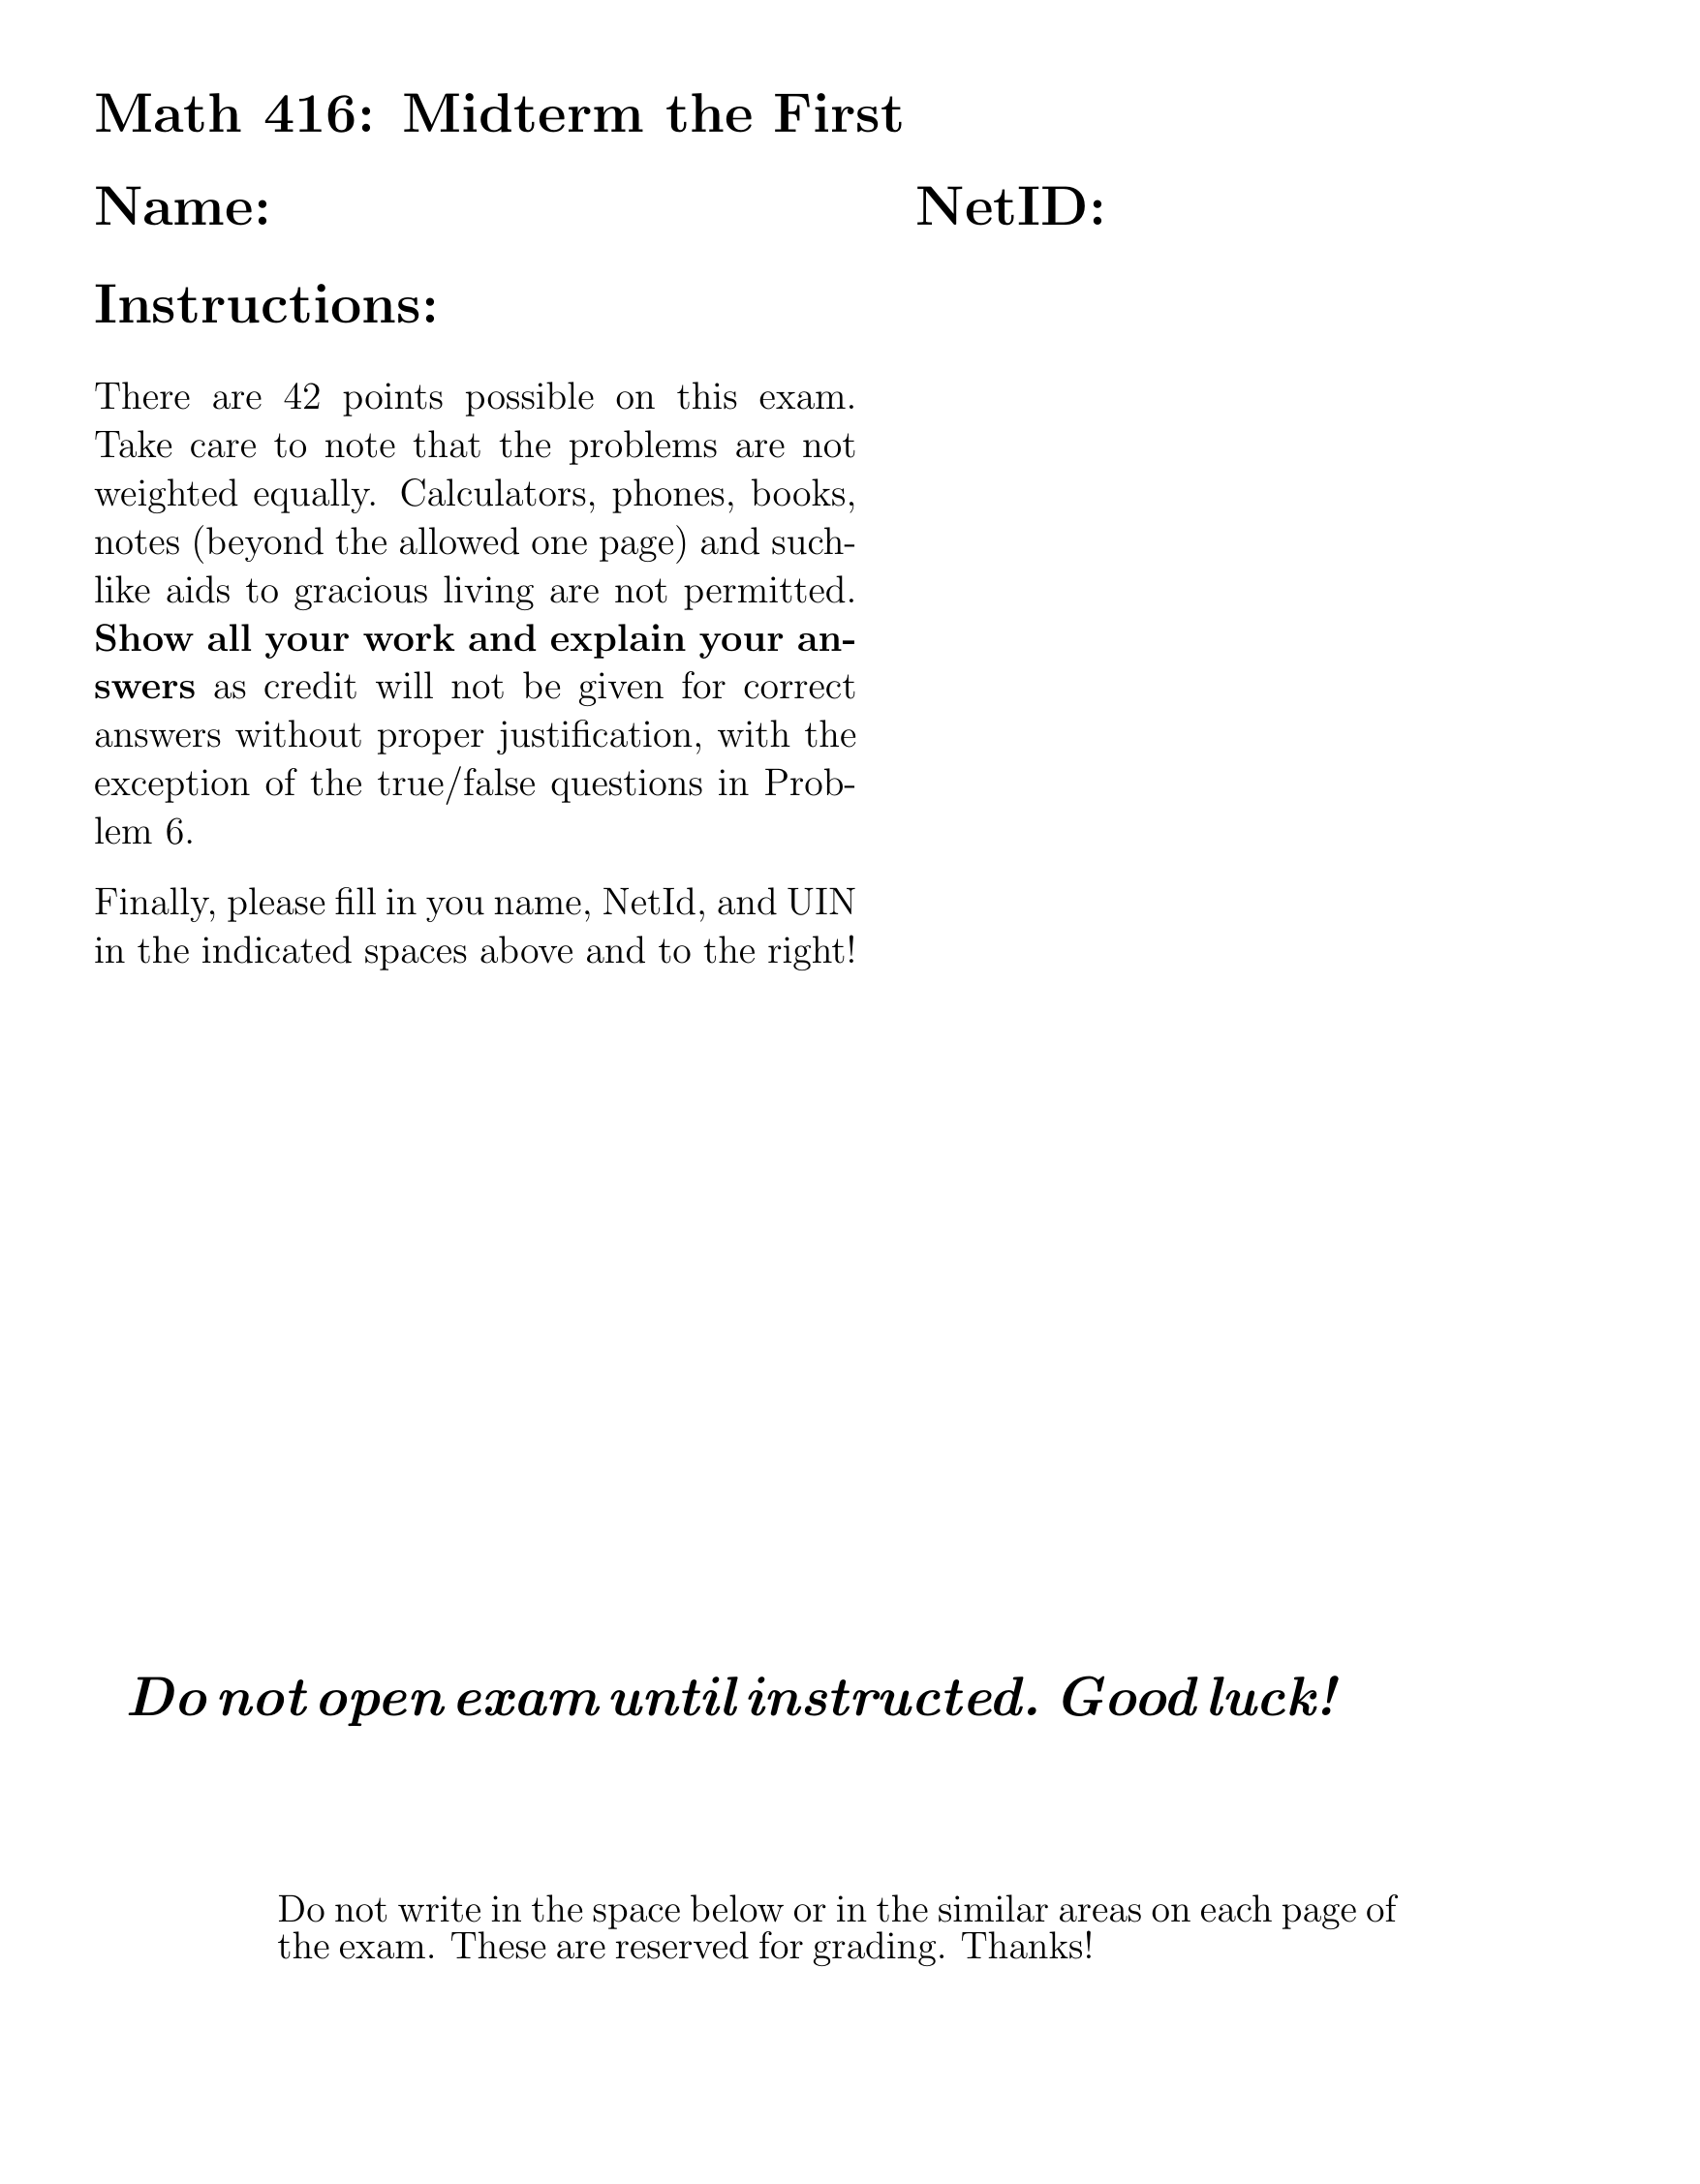
\begin{tikzpicture} 
    \expandtikztopage
    % 
    \node[below right=0.75cm] at (D) 
        {\huge \bf Math 416: Midterm the First};
    
    \node[below=2.35cm,  right=0.75cm] at (D) {\huge \bf Name:};
    \node[below=2.35cm, right=0.75cm] at (0, \y) {\huge \bf NetID:};


    \node[below=3.25cm, right=0.75cm, text width=10cm,
          anchor=north west, align=justify] at (D) {
        \huge \textbf{Instructions:}

        \vspace{0.5cm}
        
        \Large There are 42 points possible on this exam. Take care to note
        that the problems are not weighted equally. Calculators, phones,
        books, notes (beyond the allowed one page) and suchlike aids to
        gracious living are not permitted. \textbf{Show all your work and
        explain your answers} as credit will not be given for correct
        answers without proper justification, with the exception of
        the true/false questions in Problem 6.

        \vspace{0.3cm}
        
        Finally, please fill in you name, NetId, and UIN in the
        indicated spaces above and to the right!
        
      };

    % UIN entry area; uncommend the draw command to see where it will go.
    \begin{scope}[shift={(1cm, 8.25cm)}]
      \newcommand{\s}{0.8}
      %\draw[line width=1pt, color=blue!20, dashed] (0, 2.0*\s) rectangle (10*\s, -10.5*\s);
    \end{scope}

    \node[text width=19cm] at (0, -4.5) {% Below the gradebox
    };

   \node[text width=19cm] at (0, -8.0) 
      {\huge \bf \emph{Do not open exam until instructed.   Good luck!}};


   \node[text width=15cm] at (0, -11) {\Large Do not write in the space below or in the
     similar areas on each page of the exam.  These are reserved for
     grading. Thanks!};

   
  \end{tikzpicture}


\end{document}